\section{Analysis strategy}\label{chap5:analysis_strategy}

Regarding the electrons, muons, jets and \MET definition and reconstruction, the standard CMS recommendations described in Chapter~\ref{chap2} are used. The specific selections used in this analysis are briefly summarised below.

Muons are identified according to the CMS recommendations for the medium working point, with the addition of some extra cuts, as defined by the following selections:
\begin{itemize}
\item identified by the standard medium muon selection described in Sec.~\ref{sec:Objects}; \textcolor{red}{Not yet defined :)}
\item $\pt> 10$\GeV;
\item $|\eta < 2.4|$;
\item $|d_{xy}| < 0.01$\,cm for $\pt < 20$\GeV and $|d_{xy}| < 0.02$\,cm for $\pt > 20$\GeV, $d_{xy}$ being the transverse impact parameter with respect to the primary vertex;
\item $|d_{z}| < 0.1$\,cm, where $d_z$ is the longitudinal distance of the muon track in the tracker extrapolated along the beam direction.
\end{itemize}

For the muon isolation the CMS recommended particle flow isolation based on the tight working point is used, corresponding to a requirement on the isolation variable of $ISO_\mathrm{tight} < 0.15$. In addition a tracker relative isolation is also applied.

For the electron identification, the tight working point is used. In addition some additional cuts to make the selection ``trigger-safe'' are included. This is done because the electron triggers already include some identification and isolation requirements that are based on the raw detector information, while the offline selections makes use of particle flow requirements. The ``trigger-safe'' selections are defined to make the the offline identification and isolation requirements tighter with respect to the online triggers.

The simulated events are corrected for the lepton trigger, identification and isolation efficiencies measured in data using the same techniques described in Sec.~\ref{sec:Selections}.

Jets are defined clustering the particle flow objects using the anti-$k_t$ algorithm with a distance parameter of 0.4. The CHS pileup mitigation technique is used. The L1, L2, L3 and L2L3 jet energy correction described in Sec.~\ref{sec:Objects} are applied. The reject jets coming from calorimeter or readout electronics noise, the loose working point for PF jet identification is used.

The b-tagging algorithm for this analysis is chosen comparing the performances of different algorithms using simulations for signal and background contributions in the phase space defined bu the analysis kinematic requirements. More precisely, two MC samples are used, one corresponding the the \hwwllnn signal produced via the ggH production mode and another corresponding to the \ttbar process. In fact, the first sample is enriched in light jets, i.e. originating by the hadronization of light quarks like u,d,c and s quarks, while the second sample is enriched in b jets, coming from the top quark decay. The b-veto efficiency, $\epsilon_\mathrm{b veto}$, is computed separately for the two samples and for the several b tagging algorithms. To compare the b tagging performance, $\epsilon_\mathrm{b veto}$ is computed for different working points, i.e. different selections on the specific b tagging discriminator, and the results are reported in the form of a ROC curve. The ROC curves corresponding to events with 0, 1 and $\geq 2$ jets are shown in Fig.~\ref{fig:btag}.

\begin{figure}[!h]
\centering
\subfigure[$N_\mathrm{jets} = 0$]{
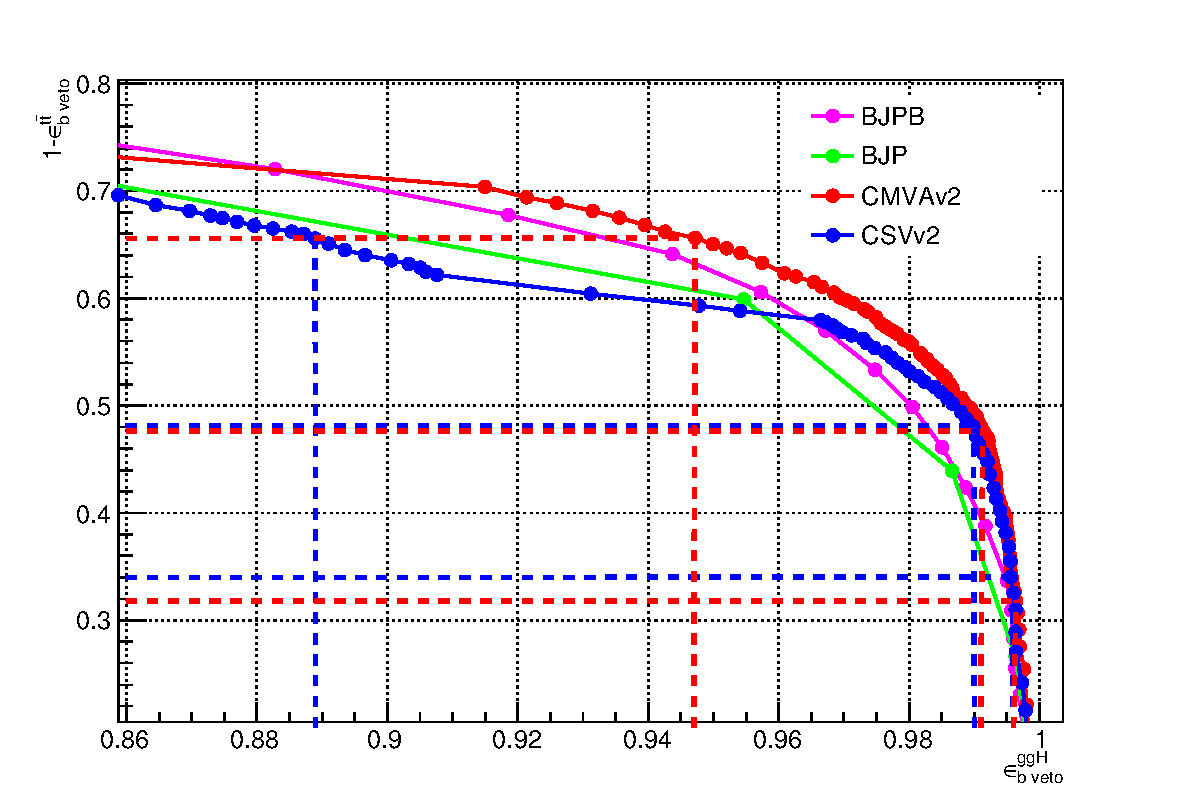
\includegraphics[width=0.45\textwidth]{images/13TeV/ROC_njet0.pdf}
}
\subfigure[$N_\mathrm{jets} = 1$]{
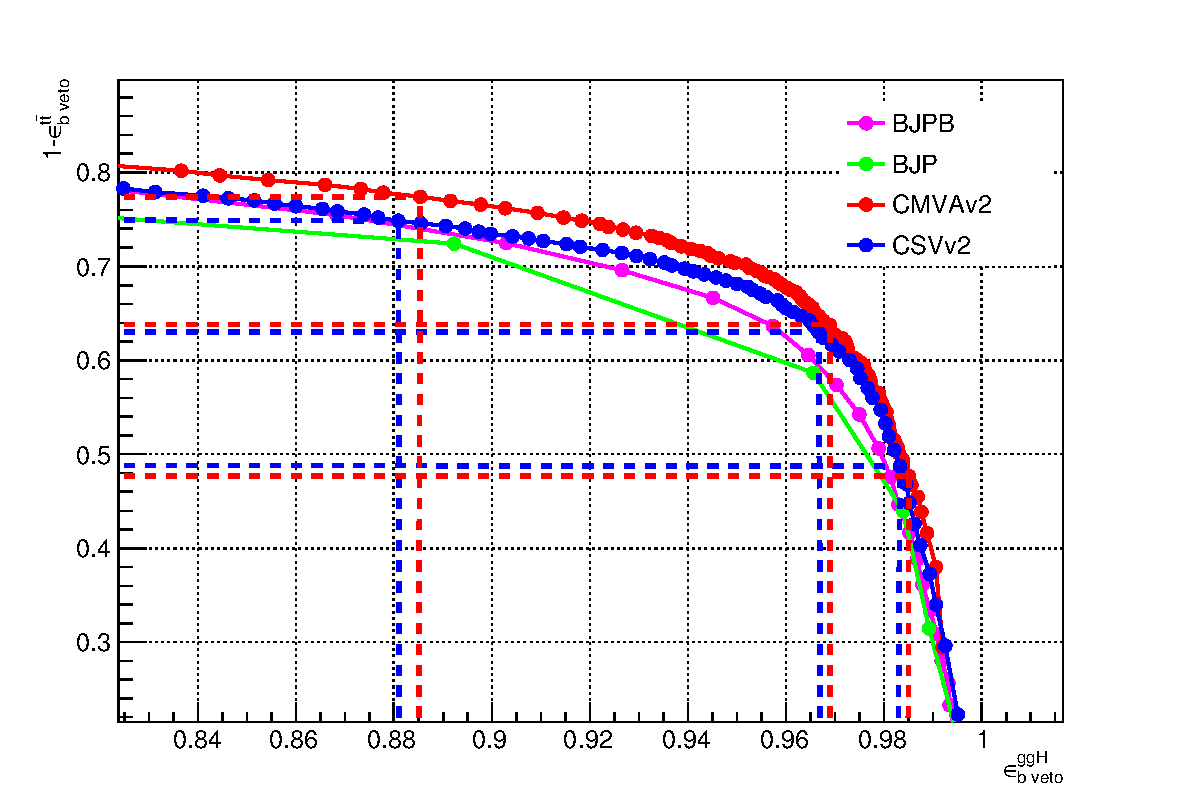
\includegraphics[width=0.45\textwidth]{images/13TeV/ROC_njet1.pdf}
}
\subfigure[$N_\mathrm{jets} \geq 2$]{
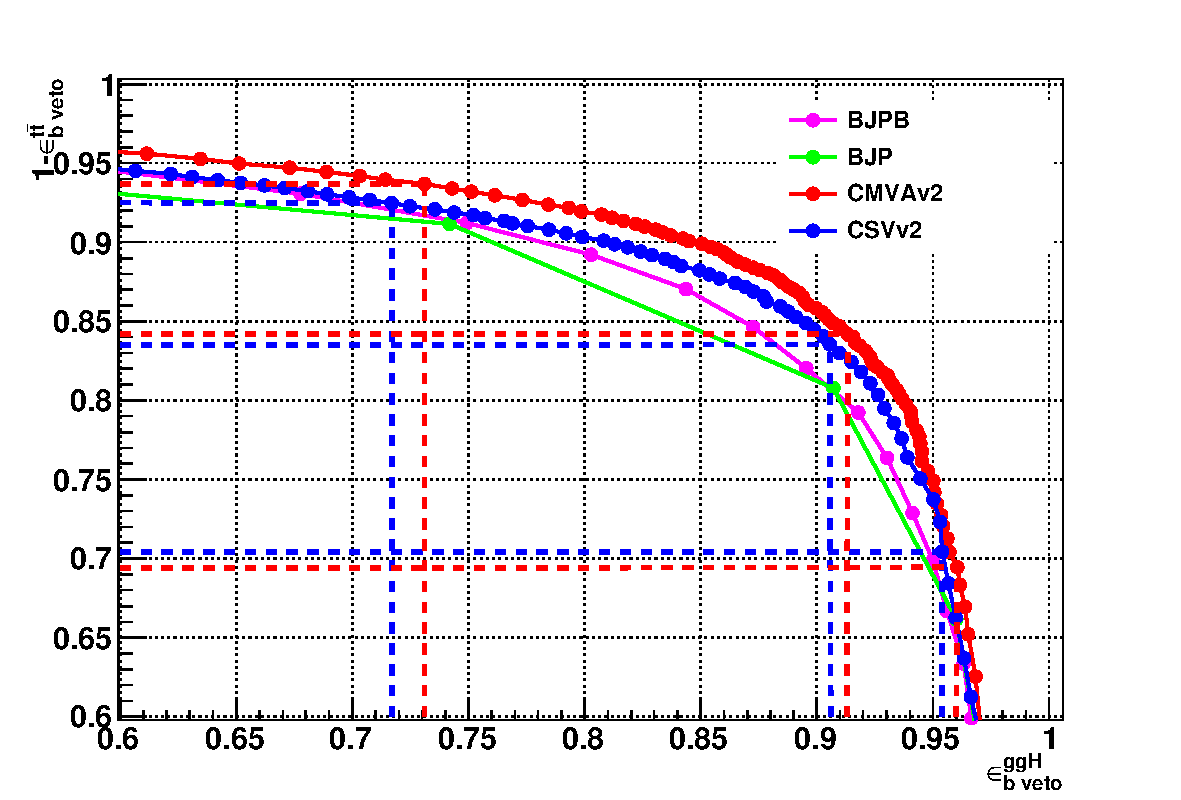
\includegraphics[width=0.45\textwidth]{images/13TeV/ROC_njetge2.pdf}
}
\caption{ROC curve for the b veto efficiency on signal and background events. The blue and red lines point out the signal efficiency and the background rejection corresponding to the three working points considered for the CSVv2 and the cMVAv2 algorithms
respectively.}\label{fig:btag}
\end{figure}






